\section{Weather symbols: quick reference}\label{p3-app:symbols}

The symbols used on the maps. Cover the right-hand descriptions and test yourself.

\begin{figure}[ht]
\centering
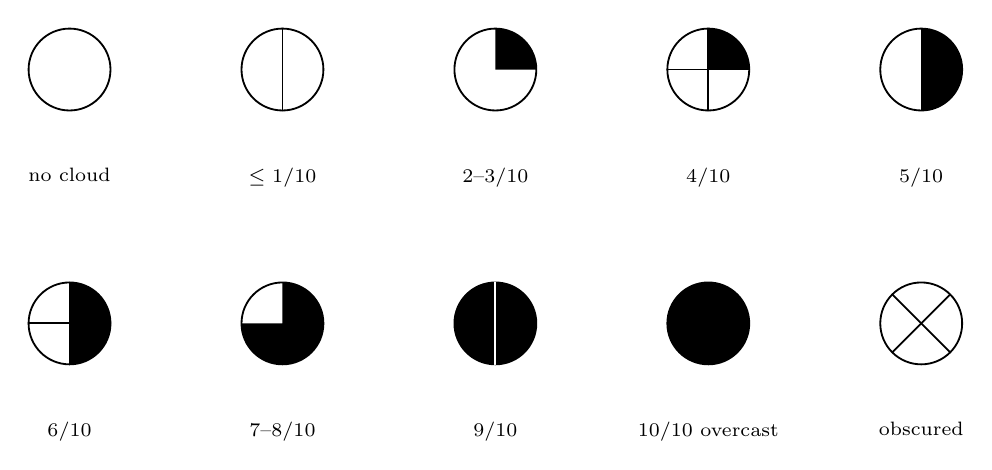
\begin{tikzpicture}[x=0.052cm,y=-0.052cm,line cap=round]\draw[black,line width=0.66pt,fill=white] (24.0,20.0) circle (10.0);
\node[anchor=north,inner sep=0pt,font=\fontsize{7.5}{7.5}\selectfont,text=black] at (24.0,44.0) {no cloud};
\draw[black,line width=0.66pt,fill=white] (76.0,20.0) circle (10.0);
\draw[black,line width=0.66pt] (76.0,10.0) -- (76.0,30.0);
\node[anchor=north,inner sep=0pt,font=\fontsize{7.5}{7.5}\selectfont,text=black] at (76.0,44.0) {$\le 1/10$};
\draw[black,line width=0.66pt,fill=white] (128.0,20.0) circle (10.0);
\fill[black] (128.0,20.0) -- (128.0,10.0) -- (129.3,10.1) -- (130.6,10.3) -- (131.8,10.8) -- (133.0,11.3) -- (134.1,12.1) -- (135.1,12.9) -- (135.9,13.9) -- (136.7,15.0) -- (137.2,16.2) -- (137.7,17.4) -- (137.9,18.7) -- (138.0,20.0) -- cycle;
\node[anchor=north,inner sep=0pt,font=\fontsize{7.5}{7.5}\selectfont,text=black] at (128.0,44.0) {2--3/10};
\draw[black,line width=0.66pt,fill=white] (180.0,20.0) circle (10.0);
\fill[black] (180.0,20.0) -- (180.0,10.0) -- (181.3,10.1) -- (182.6,10.3) -- (183.8,10.8) -- (185.0,11.3) -- (186.1,12.1) -- (187.1,12.9) -- (187.9,13.9) -- (188.7,15.0) -- (189.2,16.2) -- (189.7,17.4) -- (189.9,18.7) -- (190.0,20.0) -- cycle;
\draw[black,line width=0.66pt] (170.0,20.0) -- (190.0,20.0);
\draw[black,line width=0.66pt] (180.0,10.0) -- (180.0,30.0);
\node[anchor=north,inner sep=0pt,font=\fontsize{7.5}{7.5}\selectfont,text=black] at (180.0,44.0) {4/10};
\draw[black,line width=0.66pt,fill=white] (232.0,20.0) circle (10.0);
\fill[black] (232.0,20.0) -- (232.0,10.0) -- (233.3,10.1) -- (234.6,10.3) -- (235.8,10.8) -- (237.0,11.3) -- (238.1,12.1) -- (239.1,12.9) -- (239.9,13.9) -- (240.7,15.0) -- (241.2,16.2) -- (241.7,17.4) -- (241.9,18.7) -- (242.0,20.0) -- (241.9,21.3) -- (241.7,22.6) -- (241.2,23.8) -- (240.7,25.0) -- (239.9,26.1) -- (239.1,27.1) -- (238.1,27.9) -- (237.0,28.7) -- (235.8,29.2) -- (234.6,29.7) -- (233.3,29.9) -- (232.0,30.0) -- cycle;
\node[anchor=north,inner sep=0pt,font=\fontsize{7.5}{7.5}\selectfont,text=black] at (232.0,44.0) {5/10};
\draw[black,line width=0.66pt,fill=white] (24.0,82.0) circle (10.0);
\fill[black] (24.0,82.0) -- (24.0,72.0) -- (25.3,72.1) -- (26.6,72.3) -- (27.8,72.8) -- (29.0,73.3) -- (30.1,74.1) -- (31.1,74.9) -- (31.9,75.9) -- (32.7,77.0) -- (33.2,78.2) -- (33.7,79.4) -- (33.9,80.7) -- (34.0,82.0) -- (33.9,83.3) -- (33.7,84.6) -- (33.2,85.8) -- (32.7,87.0) -- (31.9,88.1) -- (31.1,89.1) -- (30.1,89.9) -- (29.0,90.7) -- (27.8,91.2) -- (26.6,91.7) -- (25.3,91.9) -- (24.0,92.0) -- cycle;
\draw[black,line width=0.66pt] (14.0,82.0) -- (34.0,82.0);
\draw[black,line width=0.66pt] (24.0,72.0) -- (24.0,92.0);
\node[anchor=north,inner sep=0pt,font=\fontsize{7.5}{7.5}\selectfont,text=black] at (24.0,106.0) {6/10};
\draw[black,line width=0.66pt,fill=white] (76.0,82.0) circle (10.0);
\fill[black] (76.0,82.0) -- (76.0,72.0) -- (77.3,72.1) -- (78.6,72.3) -- (79.8,72.8) -- (81.0,73.3) -- (82.1,74.1) -- (83.1,74.9) -- (83.9,75.9) -- (84.7,77.0) -- (85.2,78.2) -- (85.7,79.4) -- (85.9,80.7) -- (86.0,82.0) -- (85.9,83.3) -- (85.7,84.6) -- (85.2,85.8) -- (84.7,87.0) -- (83.9,88.1) -- (83.1,89.1) -- (82.1,89.9) -- (81.0,90.7) -- (79.8,91.2) -- (78.6,91.7) -- (77.3,91.9) -- (76.0,92.0) -- (74.7,91.9) -- (73.4,91.7) -- (72.2,91.2) -- (71.0,90.7) -- (69.9,89.9) -- (68.9,89.1) -- (68.1,88.1) -- (67.3,87.0) -- (66.8,85.8) -- (66.3,84.6) -- (66.1,83.3) -- (66.0,82.0) -- cycle;
\node[anchor=north,inner sep=0pt,font=\fontsize{7.5}{7.5}\selectfont,text=black] at (76.0,106.0) {7--8/10};
\draw[black,line width=0.66pt,fill=white] (128.0,82.0) circle (10.0);
\fill[black] (128.0,82.0) circle (10.0);
\draw[white,line width=0.66pt] (128.0,72.0) -- (128.0,92.0);
\node[anchor=north,inner sep=0pt,font=\fontsize{7.5}{7.5}\selectfont,text=black] at (128.0,106.0) {9/10};
\draw[black,line width=0.66pt,fill=white] (180.0,82.0) circle (10.0);
\fill[black] (180.0,82.0) circle (10.0);
\node[anchor=north,inner sep=0pt,font=\fontsize{7.5}{7.5}\selectfont,text=black] at (180.0,106.0) {10/10 overcast};
\draw[black,line width=0.66pt,fill=white] (232.0,82.0) circle (10.0);
\draw[black,line width=0.66pt] (225.0,75.0) -- (239.0,89.0);
\draw[black,line width=0.66pt] (239.0,75.0) -- (225.0,89.0);
\node[anchor=north,inner sep=0pt,font=\fontsize{7.5}{7.5}\selectfont,text=black] at (232.0,106.0) {obscured};
\end{tikzpicture}
\caption{Sky cover: no cloud, $\le1/10$, 2--3/10, 4/10, 5/10, 6/10, 7--8/10, 9/10, 10/10 (overcast), obscured.}
\end{figure}

\begin{figure}[ht]
\centering
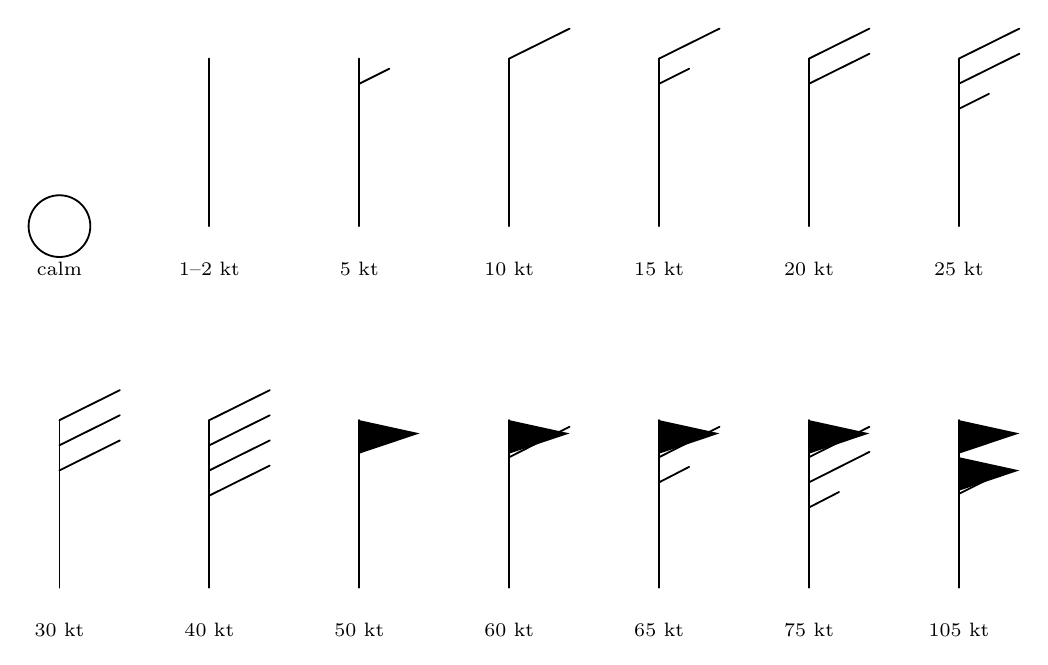
\begin{tikzpicture}[x=0.056cm,y=-0.056cm,line cap=round]\draw[black,line width=0.66pt] (24.0,52.0) circle (7.0);
\node[anchor=north,inner sep=0pt,font=\fontsize{7.5}{7.5}\selectfont,text=black] at (24.0,60.0) {calm};
\draw[black,line width=0.66pt] (58.0,52.0) -- (58.0,14.0);
\node[anchor=north,inner sep=0pt,font=\fontsize{7.5}{7.5}\selectfont,text=black] at (58.0,60.0) {1--2 kt};
\draw[black,line width=0.66pt] (92.0,52.0) -- (92.0,14.0);
\draw[black,line width=0.66pt] (92.0,19.7) -- (98.8,16.3);
\node[anchor=north,inner sep=0pt,font=\fontsize{7.5}{7.5}\selectfont,text=black] at (92.0,60.0) {5 kt};
\draw[black,line width=0.66pt] (126.0,52.0) -- (126.0,14.0);
\draw[black,line width=0.66pt] (126.0,14.0) -- (139.7,7.2);
\node[anchor=north,inner sep=0pt,font=\fontsize{7.5}{7.5}\selectfont,text=black] at (126.0,60.0) {10 kt};
\draw[black,line width=0.66pt] (160.0,52.0) -- (160.0,14.0);
\draw[black,line width=0.66pt] (160.0,14.0) -- (173.7,7.2);
\draw[black,line width=0.66pt] (160.0,19.7) -- (166.8,16.3);
\node[anchor=north,inner sep=0pt,font=\fontsize{7.5}{7.5}\selectfont,text=black] at (160.0,60.0) {15 kt};
\draw[black,line width=0.66pt] (194.0,52.0) -- (194.0,14.0);
\draw[black,line width=0.66pt] (194.0,14.0) -- (207.7,7.2);
\draw[black,line width=0.66pt] (194.0,19.7) -- (207.7,12.9);
\node[anchor=north,inner sep=0pt,font=\fontsize{7.5}{7.5}\selectfont,text=black] at (194.0,60.0) {20 kt};
\draw[black,line width=0.66pt] (228.0,52.0) -- (228.0,14.0);
\draw[black,line width=0.66pt] (228.0,14.0) -- (241.7,7.2);
\draw[black,line width=0.66pt] (228.0,19.7) -- (241.7,12.9);
\draw[black,line width=0.66pt] (228.0,25.4) -- (234.8,22.0);
\node[anchor=north,inner sep=0pt,font=\fontsize{7.5}{7.5}\selectfont,text=black] at (228.0,60.0) {25 kt};
\draw[black,line width=0.66pt] (24.0,134.0) -- (24.0,96.0);
\draw[black,line width=0.66pt] (24.0,96.0) -- (37.7,89.2);
\draw[black,line width=0.66pt] (24.0,101.7) -- (37.7,94.9);
\draw[black,line width=0.66pt] (24.0,107.4) -- (37.7,100.6);
\node[anchor=north,inner sep=0pt,font=\fontsize{7.5}{7.5}\selectfont,text=black] at (24.0,142.0) {30 kt};
\draw[black,line width=0.66pt] (58.0,134.0) -- (58.0,96.0);
\draw[black,line width=0.66pt] (58.0,96.0) -- (71.7,89.2);
\draw[black,line width=0.66pt] (58.0,101.7) -- (71.7,94.9);
\draw[black,line width=0.66pt] (58.0,107.4) -- (71.7,100.6);
\draw[black,line width=0.66pt] (58.0,113.1) -- (71.7,106.3);
\node[anchor=north,inner sep=0pt,font=\fontsize{7.5}{7.5}\selectfont,text=black] at (58.0,142.0) {40 kt};
\draw[black,line width=0.66pt] (92.0,134.0) -- (92.0,96.0);
\fill[black] (92.0,96.0) -- (105.7,99.0) -- (92.0,103.6) -- cycle;
\node[anchor=north,inner sep=0pt,font=\fontsize{7.5}{7.5}\selectfont,text=black] at (92.0,142.0) {50 kt};
\draw[black,line width=0.66pt] (126.0,134.0) -- (126.0,96.0);
\fill[black] (126.0,96.0) -- (139.7,99.0) -- (126.0,103.6) -- cycle;
\draw[black,line width=0.66pt] (126.0,104.4) -- (139.7,97.5);
\node[anchor=north,inner sep=0pt,font=\fontsize{7.5}{7.5}\selectfont,text=black] at (126.0,142.0) {60 kt};
\draw[black,line width=0.66pt] (160.0,134.0) -- (160.0,96.0);
\fill[black] (160.0,96.0) -- (173.7,99.0) -- (160.0,103.6) -- cycle;
\draw[black,line width=0.66pt] (160.0,104.4) -- (173.7,97.5);
\draw[black,line width=0.66pt] (160.0,110.1) -- (166.8,106.6);
\node[anchor=north,inner sep=0pt,font=\fontsize{7.5}{7.5}\selectfont,text=black] at (160.0,142.0) {65 kt};
\draw[black,line width=0.66pt] (194.0,134.0) -- (194.0,96.0);
\fill[black] (194.0,96.0) -- (207.7,99.0) -- (194.0,103.6) -- cycle;
\draw[black,line width=0.66pt] (194.0,104.4) -- (207.7,97.5);
\draw[black,line width=0.66pt] (194.0,110.1) -- (207.7,103.2);
\draw[black,line width=0.66pt] (194.0,115.8) -- (200.8,112.3);
\node[anchor=north,inner sep=0pt,font=\fontsize{7.5}{7.5}\selectfont,text=black] at (194.0,142.0) {75 kt};
\draw[black,line width=0.66pt] (228.0,134.0) -- (228.0,96.0);
\fill[black] (228.0,96.0) -- (241.7,99.0) -- (228.0,103.6) -- cycle;
\fill[black] (228.0,104.4) -- (241.7,107.4) -- (228.0,112.0) -- cycle;
\draw[black,line width=0.66pt] (228.0,112.7) -- (234.8,109.3);
\node[anchor=north,inner sep=0pt,font=\fontsize{7.5}{7.5}\selectfont,text=black] at (228.0,142.0) {105 kt};
\end{tikzpicture}
\caption{Wind barbs (staff pointing north, from the north): calm, 1--2, 5, 10, 15, 20, 25, 30, 40, 50, 60, 65, 75 and 105 knots.}
\end{figure}

\begin{figure}[ht]
\centering
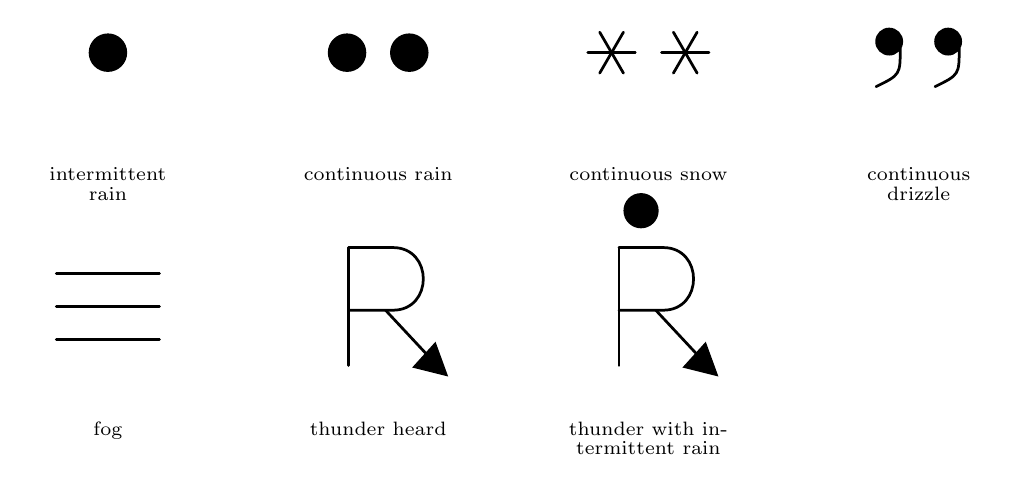
\begin{tikzpicture}[x=0.052cm,y=-0.052cm,line cap=round]\fill[black] (34.0,26.0) circle (4.7);
\node[anchor=north,inner sep=0pt,font=\fontsize{7.0}{7.0}\selectfont,text=black,align=center,text width=58pt] at (34.0,54.0) {intermittent rain};
\fill[black] (92.4,26.0) circle (4.7);
\fill[black] (107.6,26.0) circle (4.7);
\node[anchor=north,inner sep=0pt,font=\fontsize{7.0}{7.0}\selectfont,text=black,align=center,text width=58pt] at (100.0,54.0) {continuous rain};
\draw[black,line width=0.99pt] (151.2,26.0) -- (162.8,26.0);
\draw[black,line width=0.99pt] (154.1,21.0) -- (159.9,31.0);
\draw[black,line width=0.99pt] (159.9,21.0) -- (154.1,31.0);
\draw[black,line width=0.99pt] (169.2,26.0) -- (180.8,26.0);
\draw[black,line width=0.99pt] (172.1,21.0) -- (177.9,31.0);
\draw[black,line width=0.99pt] (177.9,21.0) -- (172.1,31.0);
\node[anchor=north,inner sep=0pt,font=\fontsize{7.0}{7.0}\selectfont,text=black,align=center,text width=58pt] at (166.0,54.0) {continuous snow};
\fill[black] (224.8,23.3) circle (3.4);
\draw[black,line width=0.99pt] (227.5,24.9) .. controls (227.5,31.4) .. (221.6,34.3);
\fill[black] (239.2,23.3) circle (3.4);
\draw[black,line width=0.99pt] (241.9,24.9) .. controls (241.9,31.4) .. (236.0,34.3);
\node[anchor=north,inner sep=0pt,font=\fontsize{7.0}{7.0}\selectfont,text=black,align=center,text width=58pt] at (232.0,54.0) {continuous drizzle};
\draw[black,line width=0.99pt] (21.4,79.9) -- (46.6,79.9);
\draw[black,line width=0.99pt] (21.4,88.0) -- (46.6,88.0);
\draw[black,line width=0.99pt] (21.4,96.1) -- (46.6,96.1);
\node[anchor=north,inner sep=0pt,font=\fontsize{7.0}{7.0}\selectfont,text=black,align=center,text width=58pt] at (34.0,116.0) {fog};
\draw[black,line width=0.99pt] (92.8,73.6) -- (92.8,102.4);
\draw[black,line width=0.99pt] (92.8,73.6) -- (103.6,73.6) .. controls (113.5,73.6) and (113.5,88.9) .. (103.6,88.9) -- (92.8,88.9);
\draw[black,line width=0.99pt] (101.8,88.9) -- (114.4,102.4);
\fill[black] (117.1,105.1) -- (108.3,102.9) -- (114.0,96.6) -- cycle;
\node[anchor=north,inner sep=0pt,font=\fontsize{7.0}{7.0}\selectfont,text=black,align=center,text width=58pt] at (100.0,116.0) {thunder heard};
\draw[black,line width=0.99pt] (158.8,73.6) -- (158.8,102.4);
\draw[black,line width=0.99pt] (158.8,73.6) -- (169.6,73.6) .. controls (179.5,73.6) and (179.5,88.9) .. (169.6,88.9) -- (158.8,88.9);
\draw[black,line width=0.99pt] (167.8,88.9) -- (180.4,102.4);
\fill[black] (183.1,105.1) -- (174.3,102.9) -- (180.0,96.6) -- cycle;
\fill[black] (164.2,64.6) circle (4.3);
\node[anchor=north,inner sep=0pt,font=\fontsize{7.0}{7.0}\selectfont,text=black,align=center,text width=58pt] at (166.0,116.0) {thunder with intermittent rain};
\end{tikzpicture}
\caption{Present weather: intermittent rain, continuous rain, continuous snow, continuous drizzle, fog, thunder heard, thunder with intermittent rain.}
\end{figure}

\begin{figure}[ht]
\centering
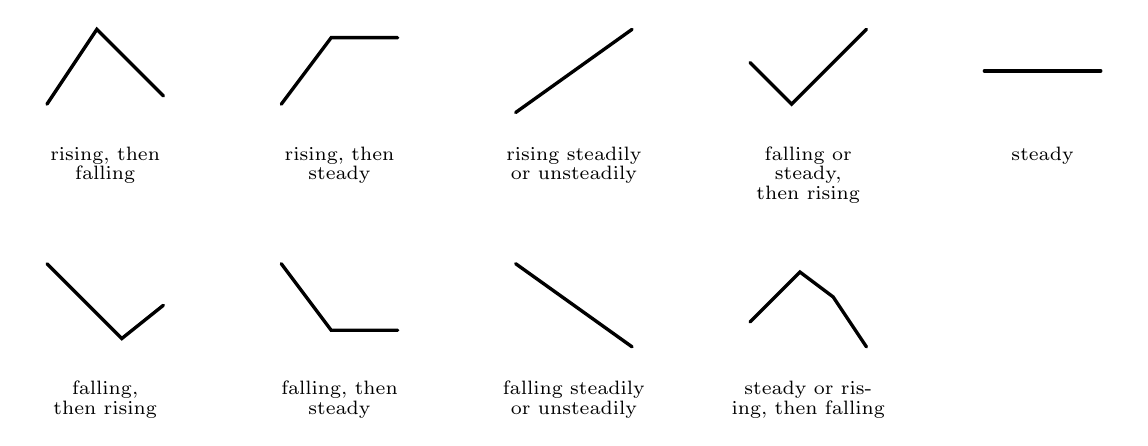
\begin{tikzpicture}[x=0.048cm,y=-0.048cm,line cap=round]\draw[black,line width=1.21pt] (12.6,32.8) -- (25.8,13.0) -- (32.4,19.6) -- (43.4,30.6);
\node[anchor=north,inner sep=0pt,font=\fontsize{7.0}{7.0}\selectfont,text=black,align=center,text width=56pt] at (28.0,44.0) {rising, then falling};
\draw[black,line width=1.21pt] (74.6,32.8) -- (87.8,15.2) -- (105.4,15.2);
\node[anchor=north,inner sep=0pt,font=\fontsize{7.0}{7.0}\selectfont,text=black,align=center,text width=56pt] at (90.0,44.0) {rising, then steady};
\draw[black,line width=1.21pt] (136.6,35.0) -- (167.4,13.0);
\node[anchor=north,inner sep=0pt,font=\fontsize{7.0}{7.0}\selectfont,text=black,align=center,text width=56pt] at (152.0,44.0) {rising steadily or unsteadily};
\draw[black,line width=1.21pt] (198.6,21.8) -- (209.6,32.8) -- (229.4,13.0);
\node[anchor=north,inner sep=0pt,font=\fontsize{7.0}{7.0}\selectfont,text=black,align=center,text width=56pt] at (214.0,44.0) {falling or steady, then rising};
\draw[black,line width=1.21pt] (260.6,24.0) -- (291.4,24.0);
\node[anchor=north,inner sep=0pt,font=\fontsize{7.0}{7.0}\selectfont,text=black,align=center,text width=56pt] at (276.0,44.0) {steady};
\draw[black,line width=1.21pt] (12.6,75.0) -- (32.4,94.8) -- (43.4,86.0);
\node[anchor=north,inner sep=0pt,font=\fontsize{7.0}{7.0}\selectfont,text=black,align=center,text width=56pt] at (28.0,106.0) {falling, then rising};
\draw[black,line width=1.21pt] (74.6,75.0) -- (87.8,92.6) -- (105.4,92.6);
\node[anchor=north,inner sep=0pt,font=\fontsize{7.0}{7.0}\selectfont,text=black,align=center,text width=56pt] at (90.0,106.0) {falling, then steady};
\draw[black,line width=1.21pt] (136.6,75.0) -- (167.4,97.0);
\node[anchor=north,inner sep=0pt,font=\fontsize{7.0}{7.0}\selectfont,text=black,align=center,text width=56pt] at (152.0,106.0) {falling steadily or unsteadily};
\draw[black,line width=1.21pt] (198.6,90.4) -- (211.8,77.2) -- (220.6,83.8) -- (229.4,97.0);
\node[anchor=north,inner sep=0pt,font=\fontsize{7.0}{7.0}\selectfont,text=black,align=center,text width=56pt] at (214.0,106.0) {steady or rising, then falling};
\end{tikzpicture}
\caption{Barometric tendency over the past three hours.}
\end{figure}
